\section{Sudoku}
\label{sec:datasets-sudoku}

The Sudoku dataset consists of $9 \times 9$ puzzles together with
their unique solutions. The graph structure of the predictor is the
constraint graph defined in Section~\ref{sec:markov-networks}, with
$|V| = 81$ nodes and $|E| = 810$ edges; the label set is
$\mathcal{Y} = \{1, \ldots, 9\}$.

\subsection{Source}
\label{subsec:sudoku-source}

Puzzles are drawn from the Kaggle dataset
\texttt{bryanpark/sudoku}~\cite{park2018sudoku}, distributed under
the CC0 license. The dataset contains roughly one million puzzle
/ solution pairs in CSV format with two columns,
\texttt{quizzes} and \texttt{solutions}, each holding an
$81$-character string of digits $0$--$9$. A character of
\texttt{0} in the \texttt{quizzes} column denotes a blank cell;
the corresponding entry in \texttt{solutions} is the digit that
the solver must recover. The full source is large, uniform in
format, publicly accessible, and permissively licensed, which
makes it a good fit for reproducible benchmarking.

The library function \texttt{ensure\_sudoku\_csv} resolves the
local CSV path automatically via the \texttt{kagglehub} downloader,
caching the file in the user's Kaggle cache directory; an
explicit \texttt{csv\_path} argument bypasses the download for
manual installations.

\subsection{Symbolic variant}
\label{subsec:sudoku-symbolic}

Each puzzle is encoded as a tensor
$x \in \mathbb{R}^{81 \times 9}$ obtained by one-hot encoding
the $81$ cells:
\begin{itemize}
    \item Blank cells (\texttt{quiz} value $0$) are mapped to the
    9-dimensional zero vector.
    \item A clue digit $d \in \{1, \ldots, 9\}$ is mapped to a
    one-hot vector with a $1$ at index $d - 1$.
\end{itemize}
The corresponding output $y \in \{0, \ldots, 8\}^{81}$ is the
solution vector with digits shifted by $-1$ to be zero-indexed,
matching the label-space convention used throughout
Chapter~\ref{chap:background}.

A typeset example puzzle is shown in
Figure~\ref{fig:sudoku-symbolic-example}: clue digits are
rendered in bold; blank cells correspond to the zero vectors above
and are filled in by the predictor at evaluation time.

\begin{figure}[htbp]
\centering
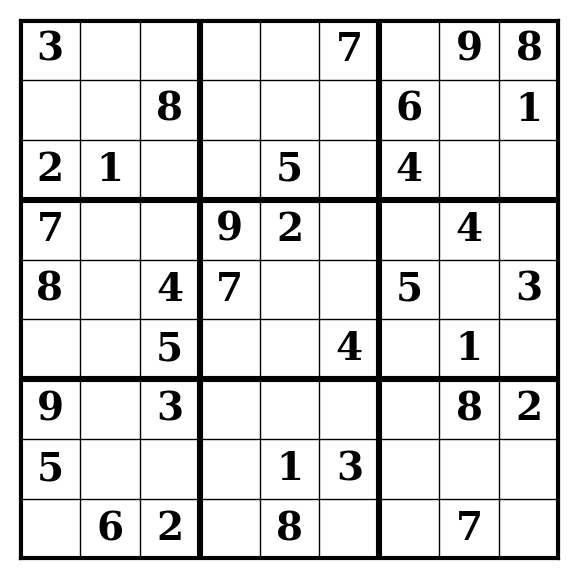
\includegraphics[width=0.45\textwidth]{figures/data/sudoku_symbolic_example}
\caption[Symbolic Sudoku example]{Example Sudoku puzzle from the
training split; clues are bold.}
\label{fig:sudoku-symbolic-example}
\end{figure}

\subsection{Visual variant}
\label{subsec:sudoku-visual}

The visual variant replaces each \emph{clue} digit by a randomly
sampled grayscale MNIST~\cite{LeCun1998} image of that digit,
drawn from a per-split image pool (Section~\ref{subsec:sudoku-splits}).
Blank cells are rendered as the all-zeros image of size
$28 \times 28$, in keeping with the symbolic encoding of a blank
cell as the zero vector. The resulting input tensor has shape
$x \in \mathbb{R}^{81 \times 1 \times 28 \times 28}$; the output
$y$ is unchanged from the symbolic case.

Figure~\ref{fig:sudoku-visual-example} shows the visual rendering
of the puzzle from Figure~\ref{fig:sudoku-symbolic-example}: each
non-blank cell carries an MNIST image of the corresponding clue
digit, with clue cells highlighted by a colored border so that
they are distinguishable from blanks at a glance.

\begin{figure}[htbp]
\centering
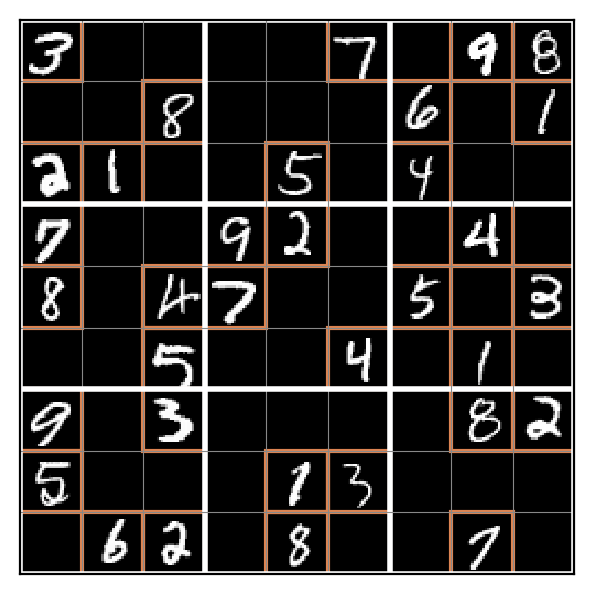
\includegraphics[width=0.6\textwidth]{figures/data/sudoku_visual_example}
\caption[Visual Sudoku example]{Visual rendering of the puzzle in
Figure~\ref{fig:sudoku-symbolic-example}; clue cells have an
orange border.}
\label{fig:sudoku-visual-example}
\end{figure}

\subsection{Splits and reproducibility}
\label{subsec:sudoku-splits}

A total of $50{,}000$ puzzles are sampled from the source CSV
with the random seed \texttt{puzzle\_seed = 42}. The sampled
puzzles are then permuted and split into $30{,}000$ training,
$10{,}000$ validation, and $10{,}000$ test puzzles.

The MNIST image used to render each clue is chosen with a
reproducible per-cell index. The pools are disjoint across
splits:
\begin{itemize}
    \item \textbf{Train.} For each digit $d \in \{1, \ldots, 9\}$,
    the training pool is the first $75\%$ of the MNIST training
    images of class $d$.
    \item \textbf{Val.} The remaining $25\%$ of the MNIST training
    images of class $d$.
    \item \textbf{Test.} The MNIST \emph{test} set images of class
    $d$ (entirely separate from train and val).
\end{itemize}
The within-split image-index assignment uses
\texttt{mnist\_seed = 200} with offsets $+0$, $+1$, $+2$ for the
train, val, and test splits respectively. All seeds are recorded in
the \texttt{config.json} written next to the data tensors, so the
benchmark is reproducible from the seeds alone.

\subsection{Statistics}
\label{subsec:sudoku-statistics}

\paragraph{Blank-cell rate.}
The Kaggle source produces puzzles with approximately $36$ given
clues on average; the empirical fraction of blank cells across
the training split is $0.5494$, consistent with the canonical
``$36$ clues out of $81$ cells'' difficulty profile.

\paragraph{Clue counts.}
Figure~\ref{fig:sudoku-difficulty} shows the histogram of the
number of clues per puzzle across the training split. The
distribution is tightly concentrated, indicating that the source
CSV is essentially a single difficulty grade rather than a mix of
difficulty levels.

\begin{figure}[htbp]
\centering
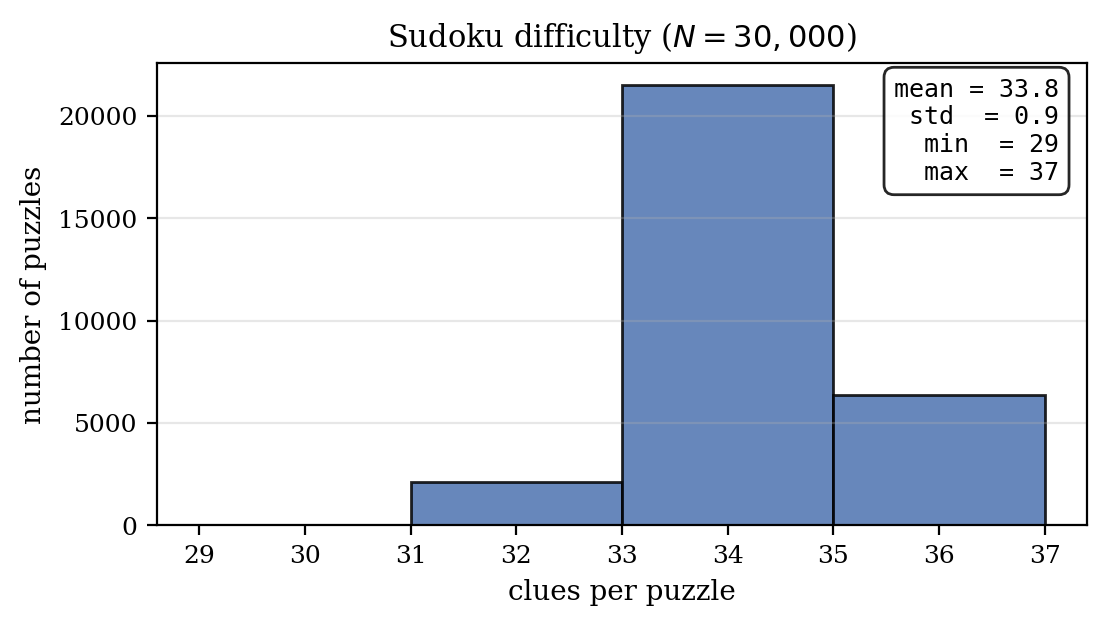
\includegraphics[width=0.85\textwidth]{figures/data/sudoku_difficulty}
\caption[Sudoku difficulty histogram]{Clue counts per puzzle,
Sudoku training split.}
\label{fig:sudoku-difficulty}
\end{figure}

\paragraph{Clue rate per cell.}
Figure~\ref{fig:sudoku-clue-rate-per-cell} shows, for every cell
$(r, c)$ in the $9 \times 9$ grid, the fraction of training
puzzles in which that cell is non-blank. The clue rate is roughly
uniform across the grid, indicating that the Kaggle source does
not preferentially clue specific cell positions.

\begin{figure}[htbp]
\centering
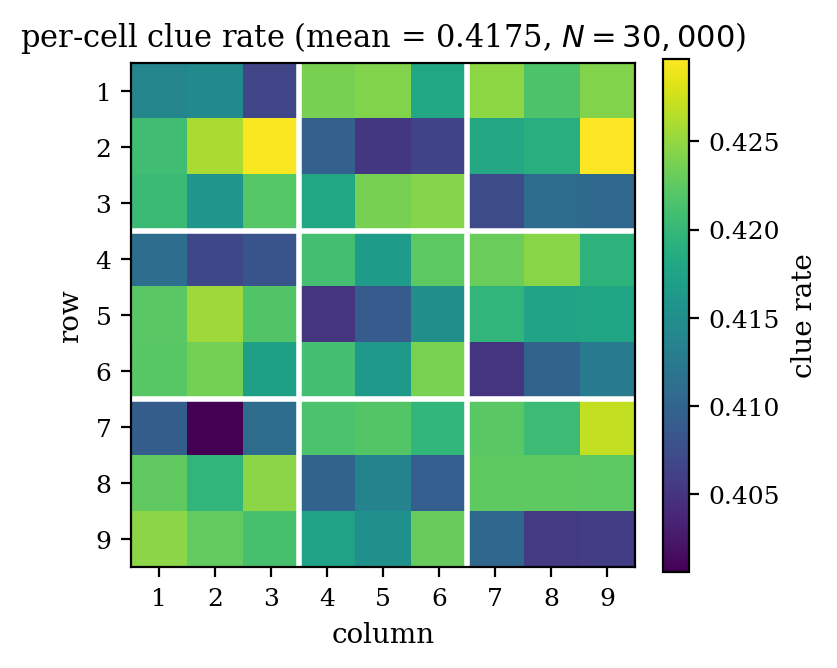
\includegraphics[width=0.55\textwidth]{figures/data/sudoku_clue_rate_per_cell}
\caption[Sudoku clue rate per cell]{Per-position clue rate on the
Sudoku training split: fraction of puzzles in which each cell
$(r, c)$ is non-blank.}
\label{fig:sudoku-clue-rate-per-cell}
\end{figure}


\paragraph{MNIST-pool reuse.}
Each puzzle has roughly $36$ clue cells distributed across the $9$
digit classes (an average of about $4$ clue cells per digit per
puzzle). Across the $30{,}000$ training puzzles this gives
$30{,}000 \times 4 \approx 120{,}000$ clue cells per digit, drawn
from only about $6{,}000$ MNIST images per digit in the training
pool. Every MNIST image is therefore reused roughly $20$ times on
average. The full per-digit distribution of reuse counts is shown in
Figure~\ref{fig:sudoku-mnist-pool-usage}; the medians are well
above zero across all digits, confirming that the pool is large
enough to avoid pathological under-coverage of any individual
image.

\begin{figure}[htbp]
\centering
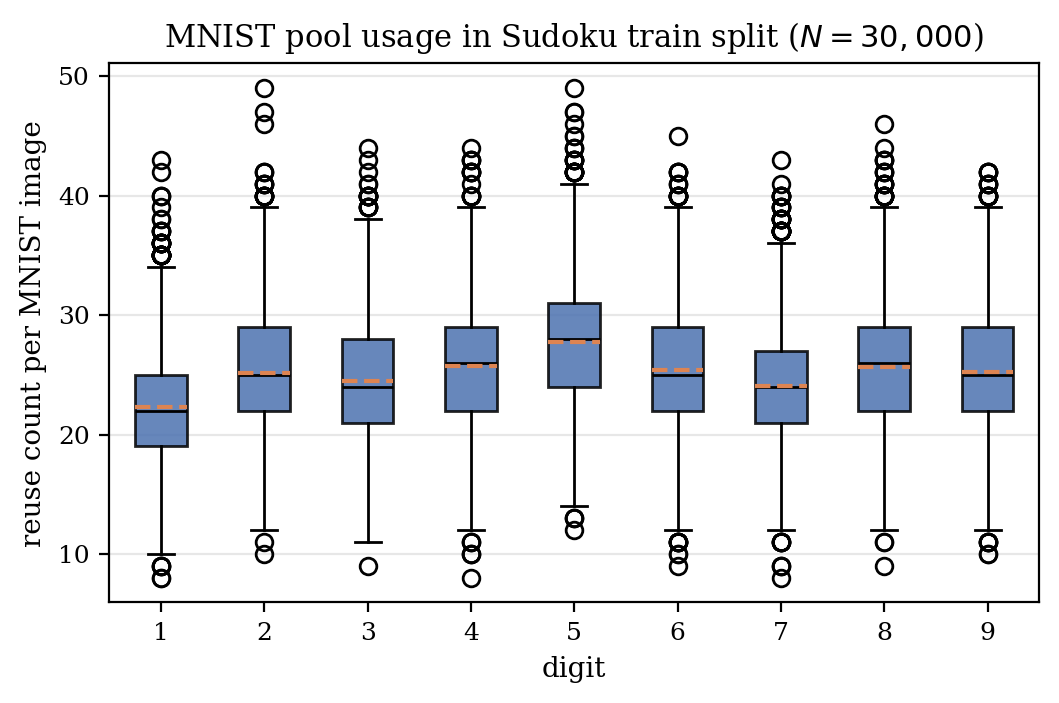
\includegraphics[width=0.85\textwidth]{figures/data/sudoku_mnist_pool_usage}
\caption[Sudoku MNIST pool usage]{Per-digit reuse counts of
training-split MNIST images.}
\label{fig:sudoku-mnist-pool-usage}
\end{figure}
